\chapter{\color{oxfordblue} The ATLAS Experiment and the LHC}\label{chapter-ATLAS}
\textit{
Modern particle physics is at the edge of the technological reach of science. To discover the Higgs boson, an extremely complex infrastuctre is required to probe physics at the required scale. The \gls{lhc} at \gls{cern} is consequently the largest and most powerful particle accelerator since its construction in 2008 \cite{LyndonEvans_2008}. It is easily ranks as one of the mox complex machine ever created. Protons are accelerated to up to 99.999999\% of the speed of light $c$, in a giant ring-shaped accelerator of 27 km of periphery. In order to steer such an energetic beam, superconducting magnets are deployed along the beamline and cooled down with liquid helium to 1.9 $K$.  These beams are made of bunches of particles, collided precisely at four specific interactions points where large detectors are built and operated by dedicated experiments: ATLAS \cite{TheATLASCollaboration_2008}, CMS \cite{TheCMSCollaboration_2008}, LHCb \cite{TheLHCbCollaboration_2008}, and ALICE \cite{TheALICECollaboration_2008}. The first two are multi-purpose experiments with overlapping physics programs, while LHCb and ALICE are respectively dedicated to flavour and heavy-ions physics. This chapter described the experimental setup of the \gls{lhc} and the ATLAS experiment.} \\ 

\section{The Large Hadron Collider}
The last machine in a complex multi-stage accelerator complex of CERN displayed in Figure \ref{fig-CernAccSys}, the \gls{lhc} is capable of frontally colliding proton or heavy ion beams. These beams are made of bunches of particles, collided precisely at four specific interactions points where large detectors are built and operated by dedicated experiments. Proton beams starts as ionised hydrogen $H^-$ passed to a linear accelerator called LINAC4\footnote{Before 2020, it was LINAC2.} to reach energies of 160 MeV. The next stage is the Proton Synchroton Booster (BOOSTER) after stripping the ionised hydrogen of its two electrons, to bring the beams to energies of 2 GeV. The protons are then passed to the Proton Synchrotron (PS) to reach energies of 26 GeV, followed by the Super Proton Synchrotron (SPS) to reach energies of 450 GeV. The beams are then injected into the \gls{lhc} for their final acceleration of up to 6.5 TeV for a total centre of mass energy of $\sqrt{s} = 13$ TeV in Run 2.  \\


The operation of the \gls{lhc} is split into dedicated \textit{runs} of data taking that are separated by \textit{shutdowns} to maintain or upgrade the infrastucture. Some key metrics from these runs at the ATLAS experiment are displayed in Table~\ref{tbl:LHCATLASperf}
\begin{table}[!htbp]
    \begin{center}
        \renewcommand{\arraystretch}{1.2}
      %\resizebox{0.99\textwidth}{!}{
        \begin{tabular}{cc|cccc} \hline \hline 
          & Year & $\sqrt{s}$ [TeV] & $\langle \mu \rangle$ &  Luminosity $\mathcal{L}$ [cm$^{-2}$s$^{-1}$] & $\int\mathcal{L}$ [fb$^{-1}$] \\ \hline
          Run 1 & 2010 - 2012 & 7-8    & 18 & 8 $\times$ $10^{33}$    & $26.4$ \\
          Run 2 & 2015 - 2018 & 13     & 34 & 1-2 $\times$ $10^{34}$  & $140$ \\
          Run 3 & 2022 - 2025 & 13.6     & 50 & 2 $\times$ $10^{33}$    & $65$ \\

          \hline\hline
        \end{tabular}
      %}
      \caption{Metrics on the accerelarator performance of the LHC in the different runs of data taking. The reported values correspond to those recorded by the ATLAS experiment \cite{ATLAS:run1Lumi, ATLAS:2022hro, ATL-DAPR-PUB-2023-001}. Numbers for the ongoing Run 3 are preliminary, with the integrated luminosity listed considering events recorded until July 2023. The number of interactions per bunch crossing averaged over each run is displayed as $\langle \mu \rangle$.} % TODO Define BL and d0
      \label{tbl:LHCATLASperf}
    \end{center}
  \end{table}

To observe quark and gluon jets as well as any other animal of this particle zoo, massive accelerator complexes and detector systems were assembled. This short introduction focuses on the ATLAS Experiment at CERN, since this project is calibrated to their data input. In Physics, energy and (inverse) length are connected, as suggested by the famous Planck-Einstein relation $E = \frac{h \, c}{\lambda}$, relating the energy $E$ to Planck's constant $h$, the speed of light in vacuum $c$ and the wavelength $\lambda$. To observe or, equivalently, to measure requires to reach a wavelength of the size of the investigated objects and therefor the right energy. The smaller the object, the larger the energy required. The interest of accelerators is precisely to increase the kinetic energy of components before ``releasing'' their content through collisions but, more generally speaking, interactions. New elements are produced from the decay of the initial particles that unveil the processes ruling Physics at the energy investigated. Most accelerators, such as the CERN's \gls{lhc}, exploit a circular shape to keep the beams of charged particles, typically gathered into bunches, in a closed trajectory while their speed (and hence kinetic energy) is increased with each revolution by the use of radiofrequency cavities. This device generates an oscillating electromagnetic field synchronised with the evolving revolution frequency of the bunches to accelerate them. The beams are constrained to their expected trajectory by powerful magnetic systems. Different geometries, such as dipoles and quadrupoles are used to monitor, control, and shape the extent of the bunches. The \gls{lhc} is only the last ring in a complex chain of accelerators, as suggested in the diagram of the CERN operation presented in figure \ref{CernAccSys}. It operates with pre-accelerated protons or \textit{ions} (atoms or molecules with a net electrical charge). 

\begin{figure}[!h]
\centering
\hspace*{-0.5in}
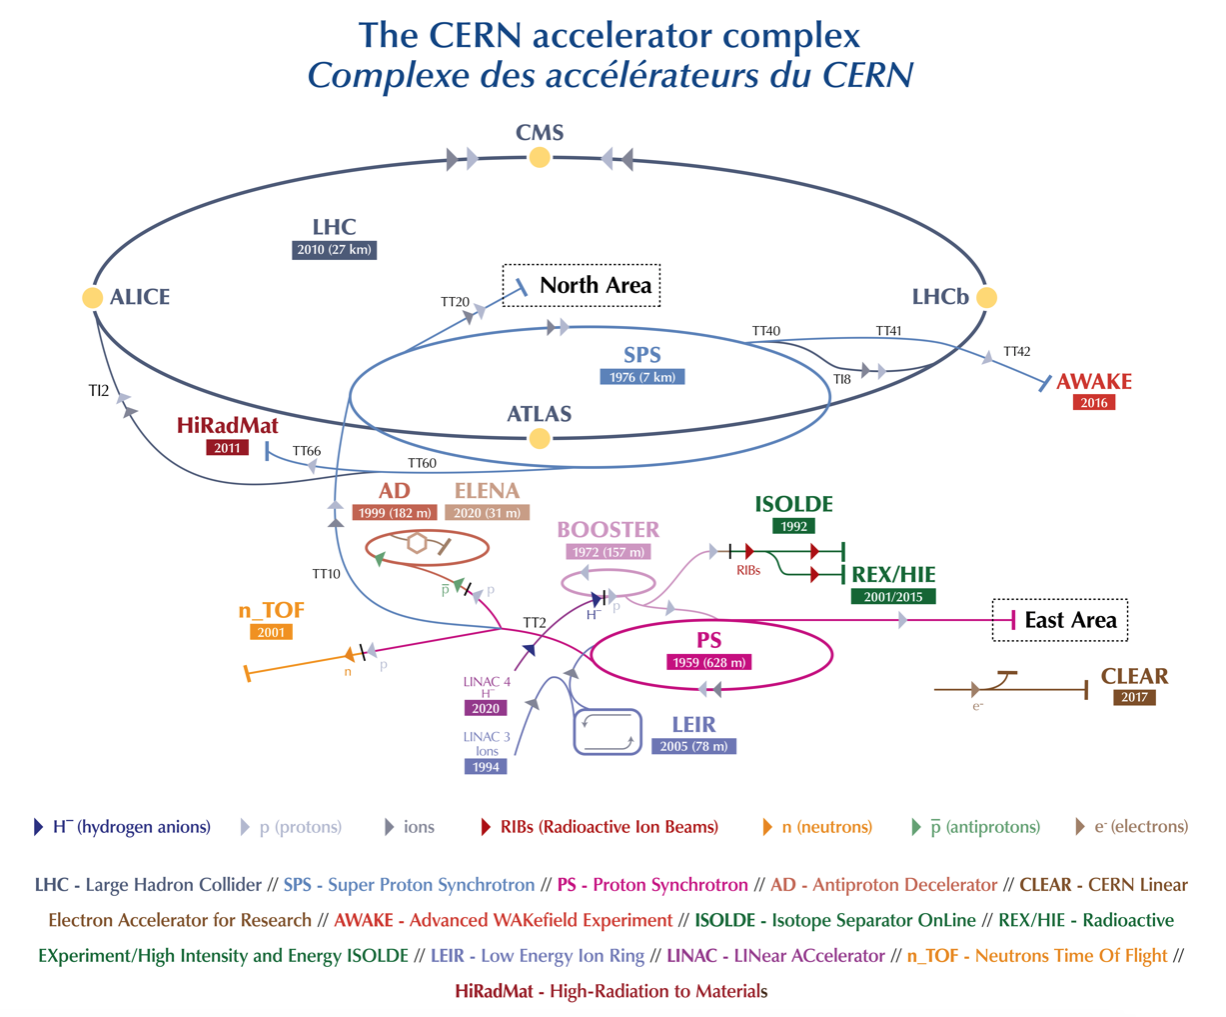
\includegraphics[scale = 0.4]{Images/ATLAS/cernAcc}
\caption{The accelerator complex of CERN during Run 2 \cite{CERNAcc}. The LHC is the top dark blue ring.}
\label{fig-CernAccSys}
\end{figure}
\newpage
Along their trajectory, two different beams can collide at a controlled \textit{\gls{ip}}. The word \textit{event} is used to encompass all information and processes emanating from the collision of two bunches (all collisions within a 25 ns period). For the purpose of this project, the collided elements in the two beams are protons at a centre of mass energy of 13 TeV, where 1 TeV = 1000 GeV. At these energies, the constituents of protons, as perceived by observing their decay, do not match the often presented and simplified three quarks picture (2 $u$ and 1 $d$). They are made of a probabilistic set of constituents called \textit{partons}. \textit{Parton distribution functions} were phenomenologically derived to quantify the probability distribution of observing a given parton at a given momentum transfer due to the interaction undergone \cite{pdfLHC}. In a sense, the content of a proton is governed by a probability distribution depending on the energy at which the proton is observed. Physicists analyse the constituents of matter arising from the collision by building giant detectors around this particular location. The ATLAS collaboration uses a cylindrically shaped multi-layered detector that is 45 m long with a diameter of 26 m and sitting in a cavern 100 m below ground, as presented in figure \ref{AtlasDec}.

\begin{figure}[!h]
\centering
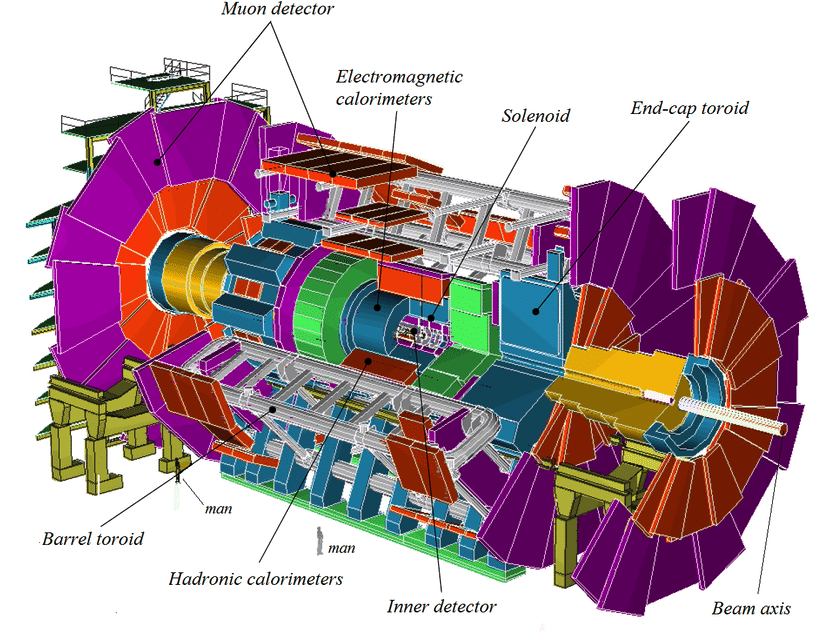
\includegraphics[scale = 0.5]{Images/ATLAS/Atlas.png}
\caption[Schema of the ATLAS detector]{Schema of the ATLAS detector \cite{AtlasWeb}.}
\label{AtlasDec}
\end{figure}

Such a detector is far more versatile than needed for the present project. This short presentation focuses on its essential components. Following a radius from the \gls{ip} (in the centre of the detector) towards the exterior, the main elements encountered are \cite{AtlasInstruDec}:
\begin{itemize}
\item An inner detector: different technologies are deployed to be sensitive to the presence of charged particles in active cells. It allows the reconstruction of a \textit{track} (a path) for electrically charged particles going through its layers, lending to the device the name of \textit{track detector} or \textit{tracker}. A variety of algorithms are employed in the ALTAS experiment to fit a track to a set of hits. A \textit{hit} is a localised deposit of energy, usually in a tracker or a calorimeter cell. A point from which new tracks emerge is called a \textit{vertex}, with the \textit{\gls{pv}} being the main vertex of the event, from which most of the interesting tracks come. 
\item A solenoid: a large cylindrical magnet releasing a magnetic field parallel to the axis of the cylinder, along the beamline. It has the effect of curving the trajectory of charged particles, as dictated by the famous Lorentz force $\vec{F} = q \vec{v} \times \vec{B} + q \vec{E}$, $q$ being the charge of the particle, $\vec{v}$ its velocity, and where $\vec{B}$, the magnetic flux density, and $\vec{E}$, the electrical field, are taken at the position of the particle. A curved trajectory in this fixed magnetic field reveals the electric charge of a particle (since a flip of $q$ changes the direction of rotation for a given $\vec{v}$). Another advantage of curving the trajectory of a charged particle with a fixed magnetic field comes from the ability to estimate its momentum $\vec{p}$ by measuring the radius of curvature $\rho$ with the relation $p = qB \rho$. Note that for a given $p$, one can control $\rho$ by adapting $B$: this is exactly what the magnetic system of the accelerator does to constrain the bunches to their expected trajectories. 
\item Calorimeters: electromagnetic (ECAL, for electrons, positrons, and photons) and hadronic (HCAL, for hadrons) calorimeters are large active volumes which purpose is to collect (most of) the energy of a passing particle. The calorimeters are structured into cells (separated into a forward region, called \textit{endcaps}, and a central region, called the \textit{barrel}). A cell collecting an amount of energy over a certain threshold is recorded as a hit. In the ATLAS experiment, groups of cells thus triggered are clustered into larger structures called \textit{topoclusters}, for topological clusters.
\end{itemize}

The reference frame adopted in the present work is introduced in figure \ref{CoorSystem}, with the two angles being the polar angle $\theta$ and the azimuthal angle $\phi$. The $x$-axis points towards the centre of the \gls{lhc} ring, the $z$-axis is taken along the beamline, and the $y$-axis closes the basis, so that the system $x-y-z$ is right-handed. Variables living in the $x-y$ plane are referred to as \textit{transversal} and added the subscript ``$_T$''. For example, the energy projected in the transverse plane is called $E_T$ and the projection of momentum $\vec{p}$ in the $x-y$ plane is $\vec{p}_T$ with a magnitude of $p_T$, the latter being a particularly important variable in \gls{hep}. Instead of the polar angle $\theta$, one often uses the pseudo-rapidity $\eta = - \log \left( \tan \frac{\theta}{2} \right)$ that maps the $\theta$ range of $[0, \pi ]$ to $[ -\infty, \infty ]$. This transformation is motivated in ultra-relativistic Physics by the closeness of the pseudo-rapidity to the notion of rapidity. The two notions are in fact equal for massless particles. Note that there is a natural limit to the range of $\eta$ to which the detector is sensitive since, at values of $\theta$ closed to 0 or $\pi$, the particle is still inside the beam pipe and cannot be detected. The geometrical ($\eta$) and dynamical ($p_T$) limitation of events observable due to the limits of the detector is called the \textit{acceptance}. It depends on the object being studied, as different subdetectors may be involved in gathering information to identify it. A typical acceptance range for $\eta$ is the range $[-3, 3]$. 

%\begin{figure}[!h]
%\centering
%\includegraphics[scale = 0.65]{Images/Coordinate_system.png}
%\caption[Coordinate system used by the ATLAS experiment]{The coordinate system used by %the ATLAS experiment. The $x$-axis points towards the centre of the LHC and the %$z$-axis is along the beamline (p symbolises a proton). For a particle of velocity $\vec%{v}$, $\theta$ is the polar angle (between $\vec{v}$ and the $z$-axis) and $\phi$ the %azimuthal angle (between the projection of $\vec{v}$ on the $x-y$ plane and the %$x$-axis). }
%\label{CoorSystem}
%\end{figure}

In operation, the enormous rate of collisions occurring in the centre of the detector (close to 40 MHz) causes a data transfer bottleneck. A set of filters must be employed to restrict data processing to events deemed of interest. These filters are called \textit{triggers} and are implemented by a hierarchical setup of electronic devices, for the lower level, and numerical methods, for the higher one, to progressively reduce the rate of events. The raw data collected that passes all steps of the triggers can then be stored in giant databases. Several layers of processing are applied to reconstruct higher-level variables, such as the energy, the mass of a particle, the tracks, and, most importantly here, the identity or \textit{tag} of the particle (e.g., gluon or quark), from low-level information, such as hits in the tracker and deposit in the calorimeter cells. Assigning a label to a particle is called \textit{tagging}. A hierarchy of increasingly processed databases for different signal regions (regions with a predominance of a specific sort of events or particles, depending on the trigger setup used when collecting the data) is then accessible to physicists. 

To analyse the data and extract the above relevant information, several techniques are employed. As the probabilistic nature of quantum physics forbids exact event-by-event analysis, one is forced to consider distributions of observables (for example the invariant mass, equal to the energy in the centre of mass of the collision). Given this stochastic aspect, \gls{mc} methods are the natural simulation tool to produce physical events as dictated by the relevant theory: this is called the \textit{generated level} \cite{Ay:2010zza}. \gls{mc} methods were in fact initially developed for this purpose, although in a more military context. The simulated events can then be passed through another layer of simulation to include the act of detection, bringing them to the \textit{reconstructed level}. For example, when two bunches collide, the detector records a set of simultaneous and overlapping events, an effect known as \textit{\gls{pu}} that needs to be added to simulations. Many reconstructed events thus produced are agglomerated into distributions, to be compared to the measured ones. Consequently, theoretical predictions can be tested against the recorded information, to search for either agreement or deviation. This is a scientifically highly efficient albeit computationally intensive process that has favoured the common pulling of resources into a worldwide computing grid and, most notably, the Web, created at CERN in 1989 and made public in 1993. 

\section{Motivation and Open Questions}\label{Section:Mot}
The previous sections introduced the landscape of the Physics experiment. The intense efforts devoted to these gigantic experiments come from the need to perform precise tests of the Standard Model and uncover traces of new Physics. For many reasons, the \gls{sm} cannot be the final theory. For example, it already fails to include gravity. Joining this interaction with the other ones is challenging, given it is extremely weak at the quantum level and only becomes somewhat significant at larger scales, due to the positive aggregation of matter. The ambitious research programme of the Particle Physics community requires several characteristics \cite{BSM_HL_LHC}: 
\begin{itemize}
\item Many events, to reduce the statistical incertitude.
\item High energies, to increase the range of processes that can occur in a collision. Currently, the average centre of mass energy of proton-proton events in the \gls{lhc} is of about 13 TeV. 
\item Fine granularity and precise methods, to improve the quality of the collected data, reconstruct more events, implement better selections, reduce the data transfer bottleneck, improve the accuracy by finer track reconstruction, and have better-aggregated information.
\end{itemize}
The first two points are regularly improved by upgrades of the components of the intricate experimental system of the CERN accelerator complex and the ATLAS detector. The final point can greatly benefit from machine learning. This has attracted a community-wide interest for these methods, with many applications already derived, particularly in classification and reconstruction (such as track fitting and pile-up removal) \cite{Deep_Learning_HEP}. 

One such effort that is of paramount importance to the advancement of research in Particle Physics is the ability to identify and discriminate jets, and in particular those associated with quarks and gluons. These objects are indeed a by-product of many different physical processes. They leave very noticeable patterns in the different subdetectors, turning them into natural and evident clues to hunt specific signals. Better \gls{qcd} and \gls{sm} measurements as well as improved and new searches for exotic physics would be the prize of a significant increase in efficiency \cite{Search_HEP_Deep_Learning}. Specifically related to the task of quark versus gluon jet discrimination, two promising analyses that would benefit greatly from an improved classifier are \cite{QG_ML_vs_Detector}:
\begin{enumerate}
\item Searches for mono-jet of dark matter in a gluon-dominated signal.
\item Searches for dijet resonances in a quark-dominated signal.
\end{enumerate}

The history of machine learning in the context of High Energy Physics is already long, beginning with \gls{mva} in the early 2000s \cite{Bhat:2010zz} to recent deep learning applications. Most importantly, in the context of jet tagging, recently explored techniques include:
\begin{itemize}
\item \glspl{bdt}: the reference method, most commonly used given its flexibility and ease of training for a relatively good performance when fed ``highly-engineered'' physical inputs \cite{QG_ML_vs_Detector, QG_Tagging_Charged}.
\item \glspl{dnn}: their performance is usually comparable to \glspl{bdt}'s, or marginally better \cite{Definition_QGJets}. It also requires engineered inputs, for competitive efficiency. 
\item Image analysis: the calorimeter surrounding the interaction point offers a natural 3D image of the jet energy deposits. This can and has been exploited in several \gls{cnn} models. The performance obtained is however not state-of-the-art for quark versus gluon discrimination, even when combined with inside information from the tracker, but it does perform slightly better than basic \glspl{bdt}'s and \glspl{dnn}'s using typical jet information \cite{QG_JET_Tagging_Image}. The significant advantage of these methods resides in the possibility to deploy them in triggers, as they only use low-level information (calorimeter hits). 
\item Junipr: a framework for unsupervised learning deploying a \gls{rnn} around a leading order model of Physics to learn the probability distribution underlying the data \cite{Junipr}. Most observables in quantum field theory are derived through perturbation theory to a certain degree or order, with the leading order being the first term. The Junipr framework offers the possibility of performing a likelihood ratio test to discriminate between different learnt distributions (from simulations) corresponding to different types of jets. Furthermore, the probabilistic model learnt when scaffolded around a factorisation tree (a tree giving a successive order to decays leading to the final state particles observed) is interpretable. In 2019, the method was proven state-of-the-art for quark versus gluon jet discrimination on a set of simulations at the generated level \cite{JUNIPER_Discrimination}. Broadly, the method relies on \gls{rnn} to learn from the succession of decays characteristic of a specific type of jet \cite{QG_RNN_tagging}. Given these qualities, the Junipr approach is the chosen paradigm for this project and is described thoroughly in section \ref{Juniprintro}.
\item Particle cloud: an adaption of point cloud considering a jet as an unordered list of final state particles. When combined with Dynamic Graph \gls{cnn} to perform complex convolution operations on the graph of final state particles, the method can achieve good performance for jet tagging problems \cite{ParticleNet}. This approach exploits recent progresses in \gls{gnn} \cite{Survey_GNN}.
\item Energy Flow Network: this method produces a set of highly-engineered features called \textit{energy flow polynomials}. They constitute a complete set of jet substructure observables, forming a discrete basis \cite{Basis_Jet_Energy_Flow}. This information can be passed to any of the previously mentioned methods (linear classifier, \gls{bdt}, \gls{dnn}, \gls{cnn}, ...) to improve its performance in the tagging and discrimination tasks \cite{Komiske2019EnergyFN, Number_Charged_Jet}. 
\item Weakly supervised learning: several papers have suggested that this learning paradigm could prove ``more physical'' \cite{Definition_QGJets}. Indeed, the assignment of a jet as emanating from a quark or a gluon parton is an inherently phenomenological one, as it does not correspond to any real physical process. The quantum world is far more complicated than the simple image this may suggest, as the contents of a proton themselves are a probabilistic mix and jets emanate from interactions within these distributions (the previously introduced parton distribution functions). Jets are assigned such a label when their orientation corresponds to that of a \textit{mother} parton momentum. What is typically called a quark or gluon jet is a specific object possessing its own properties and emanating from distinct scenarios. Therefore, rather than learning with exact labels, it has been proposed to pursue discrimination between quark- or gluon-rich distributions collected directly from the data, made of impure samples \cite{WS_taxonomy, WS_Classification_HEP, Classification_Impure_samples, Classification_no_Label_HEP}.
\end{itemize}

These various methods have been applied with different levels of success to the task of jet tagging using information from physical simulations. However, most of them are not considered in the context of a specific measuring device, as they are restricted to \textit{generated} level simulations. Measuring distorts to a certain degree (depending on the measured variables, the state of the detector at the time, ...) the underlying distribution to bring it to the \textit{reconstructed} level. It is an unavoidable consequence of interacting with the Universe at our scale. The extra-layer of simulation required to mimic the act of detection, introducing variance and blurring the descriptive power of observables, has to be accounted for when considering the level of a certain experiment, confronted to a specific way of collecting data. The aim of this project, described in the next section, is to confront a selection of these methods to the reality of the ATLAS experiment at CERN. 

\section{Objectives and Organisation}\label{Section:Obj}
From the previous section, one can conclude that there are three main ways of representing a jet: 
\begin{enumerate}
\item As a physical object, with observables describing it, such as its width, and number of constituent particles. This leads to common methods, such as \glspl{dnn} and \glspl{bdt}.
\item As an image: whether solely from the calorimeter or combined with track and other information, offering a natural ground for \glspl{cnn}. 
\item As a succession of branchings, whether ordered (factorisation tree) or unordered (particle cloud). This gives a relational point-of-view adapted to \glspl{rnn} and \glspl{gnn}.
\end{enumerate}
This project implements \glspl{dnn} and \glspl{bdt} models for benchmark and the Junipr approach from the paradigm of recurrent learning to the specific case of the ATLAS experiment. Two main research questions are explored with this subset of models: 
\begin{enumerate}
\item Is it possible to efficiently discriminate quark and gluon jets based on the low-level information delivered by the calorimeters of the ATLAS experiment? For this purpose, Junipr models are adapted to work with topocluster momenta. Junipr is chosen as it obtains state-of-the-art result on generated level simulations.
\item Is a Junipr approach competitive compared to commonly used methods when working at the reconstructed level? For this purpose, \glspl{dnn} and \glspl{bdt} models on high-level variable of reconstructed simulations are implemented. These models were chosen as they are quite common in the field and exploit engineered variables. They thus provide a natural benchmark to analyse the results of Junipr. 
\end{enumerate}
The main novel contribution of this work is to implement the Junipr model for fully \textit{reconstructed} simulations, which are intrinsically noisier than generated-level data. Indeed, reconstructed-level data suffers from the limited precision of the detecting device, pile-up, and competing processes (both reducible, if they possess different final states, and irreducible, if they do not). The second important contribution is to develop an efficient quark versus gluon jet classifier restricting to \textit{low-level} information from the detector. This final constraint, vastly complicating the task given the lower information content, is motivated by the following points: 
\begin{itemize}
\item This kind of information is that directly gathered by the detector and, therefore, the first one accessible: exploiting it efficiently is vital in the context of triggering. A precise algorithm, trained offline, could quickly perform an intelligent online selection of interesting events. 
\item Low-level information has a geometrical nature (such as the energy deposit and track hits) due to the extent and localisation of detector cells and, to a certain degree, a recurrent one (track combination and vertices, points where new tracks emanate, radiate in a tree structure from their initial point, the \gls{pv}). Many advanced \gls{ml} techniques from the previous section can exploit these patterns. 
\end{itemize}

This project is an interdisciplinary effort between the Computer Science and Particle Physics departments of the University of Oxford. The objective of this work is to serve as a concrete basis for future physics analyses by assessing the potential of new specific computational tools based on advanced \gls{ml}. Interesting steps such as interpreting the distributions obtained (except when assessing the quality of results) or searching for specific signals involving quark and/or gluon jets are not included in the present dissertation and are left for future research. Given the COVID-19 pandemic in 2020, the entire work was carried out remotely and contacts with supervisors were restricted to mostly weekly Teams meetings (sometimes at a higher frequency with Aaron O'Neill during the stages concerned with collecting the data). This has not caused any significant issues. Indeed, the CERN community, being spread all around the globe, is used to deal with such communication restrictions and have thus developed an organisational structure appropriate for remote access.

\vspace{3.5cm}

\begin{tcolorbox}[colback=oxfordblue!5,colframe=blue!40!black,title=Summary of the Chapter]
{This chapter introduces the physical context of the project. Quarks and gluons are elementary particles from the Standard Model of Particle Physics. Having a colour charge, they are sensitive to the effects described by \gls{qcd} and hadronise to form colour-less objects. This process generates large structures of successive decays called \textit{jets} and leaves a remarkable pattern in the detector of the ATLAS experiment, based on the \gls{lhc} at CERN. Jets provide a useful tool to search for and isolate specific signals in the collected data to compare to theoretical predictions. A review of current methods introduces different machine learning-based techniques to discriminate quark from gluon jets. Among them, the Junipr framework is the most promising option, given it leads to state-of-the-art performance at the generated level and is interpretable when founded upon a physical factorisation model. This project studies an adaptation of the Junipr approach to use low-level calorimeter information to improve the accuracy at the reconstructed level of the quark versus gluon jet discrimination task. \gls{bdt} and \gls{dnn} models serve as benchmarks, given their popularity in the field and reliance on high-level variables.}
\end{tcolorbox}
